%%%%%%%%%%%%%%%%%%%%%%%%%%%%%%%%%%%%%%%%%%%%%%%%%%%%%%%%%%%%%%%%%%% 
%                                                                 %
%                            CHAPTER FOUR   - A More Sophisticated Agent- Version 2            %
%                                                                 %
%%%%%%%%%%%%%%%%%%%%%%%%%%%%%%%%%%%%%%%%%%%%%%%%%%%%%%%%%%%%%%%%%%% 
 
\chapter{Version 2 -- A More Intelligent Agent}

In this chapter, we describe Version 2 of the CFE Agent, enhanced with improved algorithms for locating the relevant section(s) of the CFE Manual for each question.  Version 1 of the CFE Agent is limited to coarse-grained sections as defined by the question sections of the CFE Exam and Manual.  Unfortunately, these sections of the manual are effectively so large, it's difficult for the agent to drill down to the text \emph{directly} related to a given question.  For intellectual-property-theft questions, for example, the ``Theft of Intellectual Property" section of the manual is 89 pages long.  For any question on this topic, pulling the entire section of the CFE manual will assure that the answer sought lies somewhere within our target document.  But with 89 pages of text in the section, we might still get the answer wrong.  Version 2 refines the filtering algorithm to help avoid this problem.



This chapter is laid out as follows:  First, we review the basic elements of Information Retrieval, the branch of AI dealing with retrieving documents from within a large collection related to an information need.  Next, we explore the open source software, Lucene, an Apache sofware program that provides information retrieval functionality.  This package was used in the implementation of Version 2 of the CFE agent.  Then, we look at the method used to break up the CFE manual into finer-grained sections, leveraging the table of contents and text metadata as means for dividing up the text along reasonable semantic lines into a collection of documents.  And finally, we present the analysis performed of a set of algorithms implemented in Version 2 using these information retrieval tools and this document collection.

One note before proceeding:  The terms, ``training set" and ``test set" are used throughout this chapter in reference to the battery of questions against which the algorithms discussed below were applied.  Indeed, we talk repeatedly about testing our algorithms against the training set, specifically. It is important to note here that ``training set" is a term of convenience in this chapter, and not one that should be taken to suggest a set for which we've optimized parameters vis \`a vis machine learning.  In fact, the algorithms we discuss in this chapter involve no training, per se, and so, it is perfectly valid to measure or test the performance of each of these algorithms against the ``training set".   (In chapter 5, however, we \emph{do} employ machine learning, and the training set and test set are used according to their conventional definition.)  Lastly, it should be mentioned that at the end of this chapter, we use the performance of each algorithm on the questions of the training set to determine the optimal algorithm to use on each question in the test set in order to measure overall performance of Version 2 of the agent.

Finally, before moving any further, during the development of Version 2, a deeper review of the definition-type questions was in order.  Some questions were re-classified according to finer grained criteria, including the following:  Nine questions were reclassified as ``I, II, III, and IV" type.  Six questions for which ``Any of the Above" was an option were re-classified as ``All of the Above" type.  There were 26 questions whose answers weren't derived from the Fraud Examiners Manual but instead from a different text, The Corporate Fraud Handbook.  Finally, five questions were re-classified as ``NOT" questions.  After reclassifying these questions, we were left with 150 definition questions in our training set upon which to base our algorithm performance analysis, reduced from our original 196 questions used for Version 1.


\section{Information Retrieval}

Information Retrieval (IR) is the branch of AI dealing with the creation of software that retrieves documents of an unstructured nature from among a large collection of documents in response to an information need expressed as a natural language query \cite{manning_2008_introduction_ch1}.   A document is a unit of data, typically unstructured or semi-structured, and typically expressed in natural language.  (One of the fundamental questions to consider in IR is how to define a document - a sentence? a paragraph? a chapter?  The answer typically depends on the nature of the problem domain.)  A document collection is simply a collection of such documents, as defined above.  Finally, a vocabulary, $V=\{t_1,t_2,t_3,...,t_n\}$ is the set of all terms over which the contents of the documents are defined.

\subsection{Boolean Retrieval}

Boolean information retrieval is based on the idea of dividing up the document collection into two sets for each query - one set of documents which meets the requirements of the boolean query and the other set whose documents does not.  Boolean queries are structured as conjunctions of disjunctions; that is, of the form of query, $q$, where

%\begin{gather*}
%q = (W_i \lor W_k \lor ...) \land ... \land (W_j \lor W_s \lor ...) \\
%\textrm{where}\ W_i = t_i, W_k = t_k, W_j = t_j, W_s = t_s, \\
%\textrm{or}\ W_i = NON\ t_i, W_k = NON\ t_k, W_j = NON\ t_j, W_s = NON\ t_s \\
%\text{where $t_i$ means that $t_i$ exists in the document and $NON\ t_i$ means it does not}
%\end{gather*}

\begin{equation}
q = (W_i \lor W_k \lor ...) \land ... \land (W_j \lor W_s \lor ...) \\
\end{equation}
where $W_i = t_i, W_k = t_k, W_j = t_j, W_s = t_s,$ or $W_i = NON\ t_i, W_k = NON\ t_k, W_j = NON\ t_j, W_s = NON\ t_s$ and where $t_i$ means that $t_i$ exists in the document and $NON\ t_i$ means it does not \cite{wiki:boolean_retrieval}.

%q = (Wi OR Wk OR ...) AND ... AND (Wj OR Ws OR ...)
%
%where Wi=ti, Wk=tk, Wj = tj, Ws = ts, or Wi = NON ti, Wk = NON tk, or Wj = NON tj, or Ws = NON ts, 
%
%where ti indicates the term ti is present in the doucument and NON ti indicates it is not.

\subsubsection{Term-Document Incidence Matrix}

Boolean retrieval may be  implemented using a data structure called a term-document incidence matrix, $A$, where $A$ is a two-dimensional array in which the $i$th row denotes the $i$th document in the document collection and where $j$th column denotes the $j$th term in the vocabulary, and where $A[i,j] = 1$ if the term, $i$ exists in the document, $j$, and 0 otherwise.  Based on $A$, the processing of a query involves finding those documents for which there is a 1 in each of the rows corresponding to the terms of the query \cite{manning_2008_introduction_ch1}.  

A significant pitfall of this method is that it requires a vast amount of memory.  Consider an example consisting of 1 million documents and a vocabulary of 500,000 words.  Then, the size of the matrix is 50 trillion (1 million x 500,000).  This matrix is also highly sparse since any given document has on average a small number of words relative to the size of the vocabulary.  Suppose, for example, each document has 1,000 words.  Then, for each document, among the 50,000 elements in its corresponding row of the matrix, only 1,000 (2\%) are non-zero \cite{manning_2008_introduction_ch1}.	

\subsubsection{Inverted Index}

An alternative implementation for boolean retrieval utilizes an inverted Index -- a hash table in which the keys are the terms in the vocabulary and the value is a linked list of all of the identifiers for those documents in which that term appears.  This technique exploits the sparsity of the term-document matrix -- requiring memory only for those elements in which $A(i,j) = 1$ \cite{manning_2008_introduction_ch1}.


\subsection{Ranked Retrieval}

Boolean retrieval has the unfortunate drawback of returning a set of documents in response to a query as a set of equally ranked units through which the user must sift in order to find the information sought \cite{manning_2008_introduction_ch6}.  Sometimes, this sifting can be sizable task depending on the number of documents returns from the boolean query.  Ranked retrieval, on the other hand, is IR in which documents are ranked according to a score that measure the degree of similarity between the query and the terms of the document and in which documents are returned in decreasing sorted order of this score \cite{manning_2008_introduction_ch6}.  

The Vector Space model (VSM) \cite{manning_2008_introduction_ch6} is one approach to ranked retrieval, and is based on representing the documents in the collection and the query as vectors and where documents are scored according to a measure of similarity between their vector representations and that of the query.  There are a number of measures, or weights, that are typically incorporated into a vector representation as discussed below.

The log of the term frequency, $\textrm{log}_{10}(tf)$ is a measure of the number of occurences of a particular term in the document.  (The log is used as opposed to the term frequency, itself, in order to dampen the effect for each additional occurrence of a term.)  The log-frequency weight of term, $t$ in document, $d$ is given by \cite{manning_2008_introduction_ch6}:

\begin{equation}
w(t,d) = 1 + \textrm{log}_{10}(tf_d), \textrm{where}\ tf_d > 0, 0\  \textrm{otherwise}
\end{equation}

Inverse document frequency is a measure of the relative scarcity of a term in a document relative to the other documents in the collection.  A higher weight is assigned to a term that appears in relatively few documents compared with one that appears in many.  The inverse document frequency, $idf(t)$, can be calculated for each term, t, of the query as follows \cite{manning_2008_introduction_ch6}:  

\begin{equation}
idf(t)  = \textrm{log}_{10}(N/df_t),
\end{equation}

\noindent
where $N$ is the number of documents in the collection and $df_t$ is the number of documents containing term, $t$.  Again, as is the case for term frequency, the log is used here to moderate the effect of the measure.

We can combine these two measures such that for each term, $t$, in each document, $d$, we have \cite{manning_2008_introduction_ch6}:

\begin{equation}
w(t,d) = (1 + \textrm{log}_{10}(tf_d)) \times \textrm{log}_{10}(N/df_t).
\end{equation}

\noindent
The vector representation of a document, $d$, is $\vec{d}$, where

\begin{equation}
\vec{d} =  [w(t_1,d), w(t_2,d), w(t_3,d),...., w(t_n, d)], 
\end{equation}

\noindent
where, as defined above our vocabulary, $V=\{t_1,t_2, ..., t_n\}$.  Note, queries can also be vectorized in the same way.  

In order to measure the relative relevance of document, $d$, to the query, $q$, the vector representations of both $d$ and $q$, $\vec{d}$ and $\vec{q}$, are harnessed to compute a quantitative measure of the level of similarity between the two vectors using the concept of cosine similarity.  Informally, the cosine similarity of two n-dimensional vectors is a measure of the cosine of the angle between them in n-dimensional space.  Normalization of the lengths of the vectors is also incorporated into this calculation to assure that longer documents' weights do not outsize the weights of shorter (but perhaps, similar) documents, (such as the query itself, which is commonly much shorter than the document against which it is compared).  

\begin{equation}
\begin{split}
\textrm{sim}(q, d) & = \dfrac{\vec{q} \cdot \vec{d}}{|\vec{q}||\vec{d}|} \\
 & = \dfrac{\vec{q}}{|\vec{q}|} \cdot \dfrac{\vec{d}}{|\vec{d}|}
\end{split}
%	= q(arrow)/length(q(arrow)) dot d(arrow)/length(d(arrow)) = 
%	= sum(i to length(V))q(i)d(i)/(sum(i to length(V)q(i)\^2))(sum(i to length(V)d(i)\^2))
\end{equation}

\noindent
For a document, $d$ whose length-normalized-vector representation is similar to that of $q$, the angle between its vector and that of $q$ should be small (close to 0), and thus have a cosine near 1.  For those documents not similar to $q$, the cosine measure will tend toward 0, (note that all of the terms in these vector-representation vectors are greater than or equal to 0).  Under the document vectorization approach, the highest $K$ documents are returned in response to a query, $q$, in order of decreasining cosine similarity, where $K$ is an arbitrary figure intended to limit the size of the return set.




\section{Transforming the CFE Manual into a Document Collection}

The CFE Manual is structured as a text book. As such, it is structured hierarchically, as most textbooks are, complete with features embedded in the text that make this hierarchy apparent.  The most obvious feature is the table of contents (TOC) and headings embedded in the text for each of the chapters, sections, subsections, and so on.  In fact, the CFE Manual has a number of tables of contents, including a main table of contents, at the front of the manual, and a set of area-specific TOCs - one for each of the major test areas - Financial Transactions and Fraud Schemes, Law, Investigation, and Fraud Prevention and Deterrence.  Fig.~\ref{fig:cfe_manual_toc} shows a section of the TOC relating to Financial Statement Analysis, a topic contained in the are of Financial Transactions and Fraud Schemes.  The summary TOC combined with the area-specific TOCs combined with text features (capitalized sub-sub-sub section titles within the text itself) were all used to programmatically break up the manual into a hierarchical structure of documents.  Fig.~\ref{fig:document_collection} shows a portion of this document structure, where on the left we see the Bankruptcy Fraud subsection, a subtopic of Financial Transactions and Fraud Schemes, and the breakdown of documents, each of which named according to a numeric identifier and a title corresponding to a title for the subsection, along with indentation showing its level in the document tree.  On the right side, we see the contents of one of the documents covering the subtopic of Bankruptcy Court.  Notice that in each document we have not only the text of the section but also a a title field (Bankruptcy Court), a question section field (Financial Transactions and Fraud Schemes), a path giving the sequence of section titles starting from the root node of the CFE manual hierarchy to the current document, and finally, the stemmed contents of the document, using the Porter Stemmer algorithm.  All of these elements were compiled for each document as possible inputs to algorithms developed downstream for answering questions.  

\section{Lucene -- A Tool for Information Retrieval}

Lucene, \url{https://lucene.apache.org/}, is a highly popular Apache software product that implements IR using a combination of Boolean Retrieval and the VSM \cite{McCandless:2010:LAS:1893016_ch1,McCandless:2010:LAS:1893016_ch2,McCandless:2010:LAS:1893016_ch3,McCandless:2010:LAS:1893016_ch4}.  First, it narrows the document set using boolean retrieval, and then it ranks the remaining documents using VSM.  The algorithms described below were implemented using this tool.  

\begin{figure}
\centering
\vspace{1.0in}
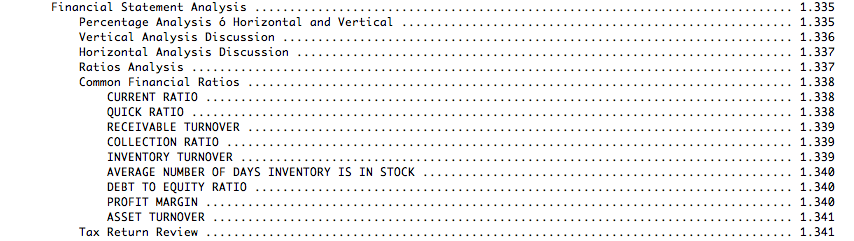
\includegraphics[width=150mm]{cfe_manual_toc.png}
\caption{A section of the table of contents from the CFE Manual}
\label{fig:cfe_manual_toc}
\end{figure}

\begin{figure}
\centering
\vspace{1.0in}
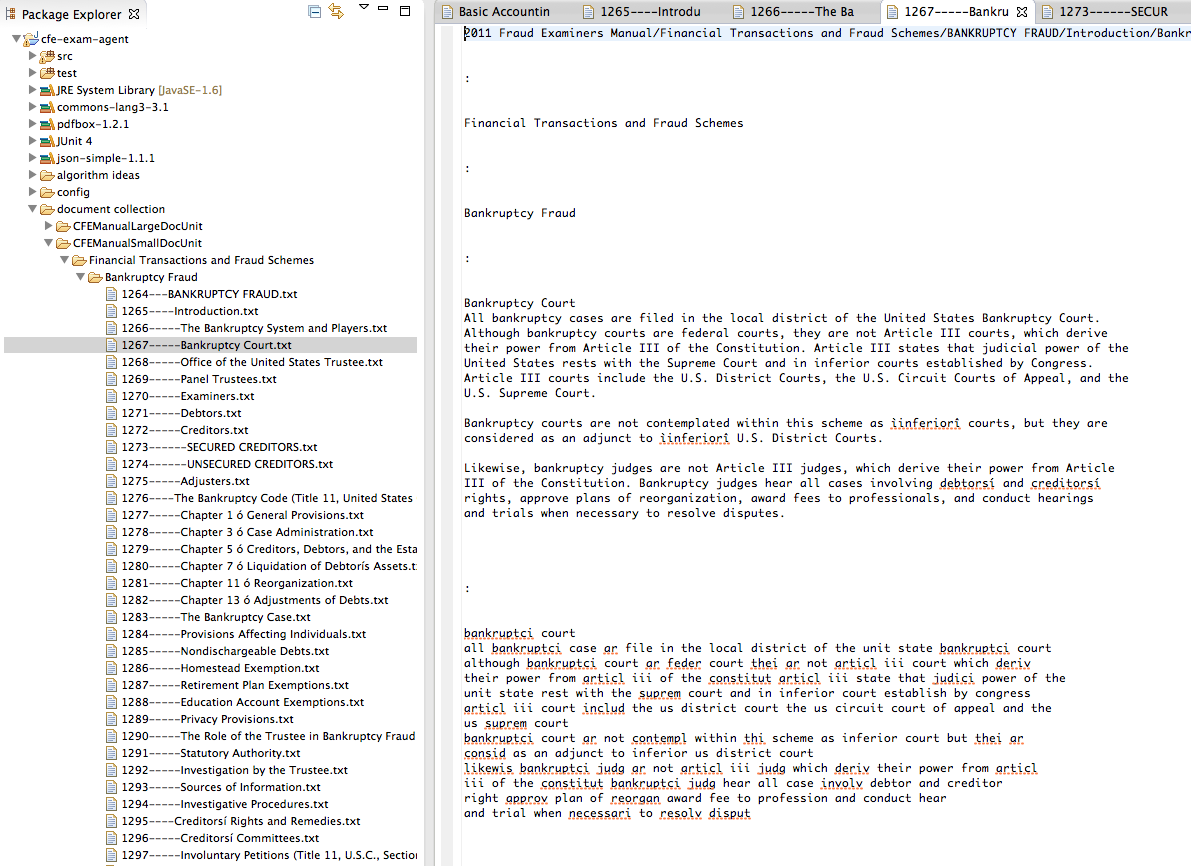
\includegraphics[width=150mm]{document_collection.png}
\caption{The CFE Manual as a Document Collection}
\label{fig:document_collection}
\end{figure}

However, before implementing any algorithms, the document collection into which the CFE manual was decomposed was indexed using the Lucene software.  Indexing is the process of essentially creating files containing the underlying data stuctures required by Lucene's combined boolean retrieval/VSM retrieval algorithm, including an inverted index for the collection and document vectorization data.  In fact, Lucene indexes were created for each question section of the manual, where each question section contains the documents from which an answer to a question pertaining to the material in that section.  When implementing the QA algorithms discussed below, the first step to any of these algorithms was locating the proper index within which to search for relevant documents, based on the exam section/question section that corresponds to the question at hand.  Fig~\ref{fig:lucene_indexes} shows a portion of the lucene indexes created by this process.  Notice that for each question section within each exam section, there are three binary files created by the lucene indexer component that contain the inverted index and document vectorization information required for the query processing component to be used in the algorithms discussed below.

One other thing of note is that as part of this process, the contents field and the title field were stemmed according to the Porter Stemmer algorithm.  Stemming is a form of semantic normalization, where words offering different senses of the same semantic unit are transformed so that they are treated as equivalent during the document scoring computation in the IR process.  For example, different words for run - run, ran, running - are all considered semantically equivalent as a result of stemming.

\begin{figure}
\centering
\vspace{1.0in}
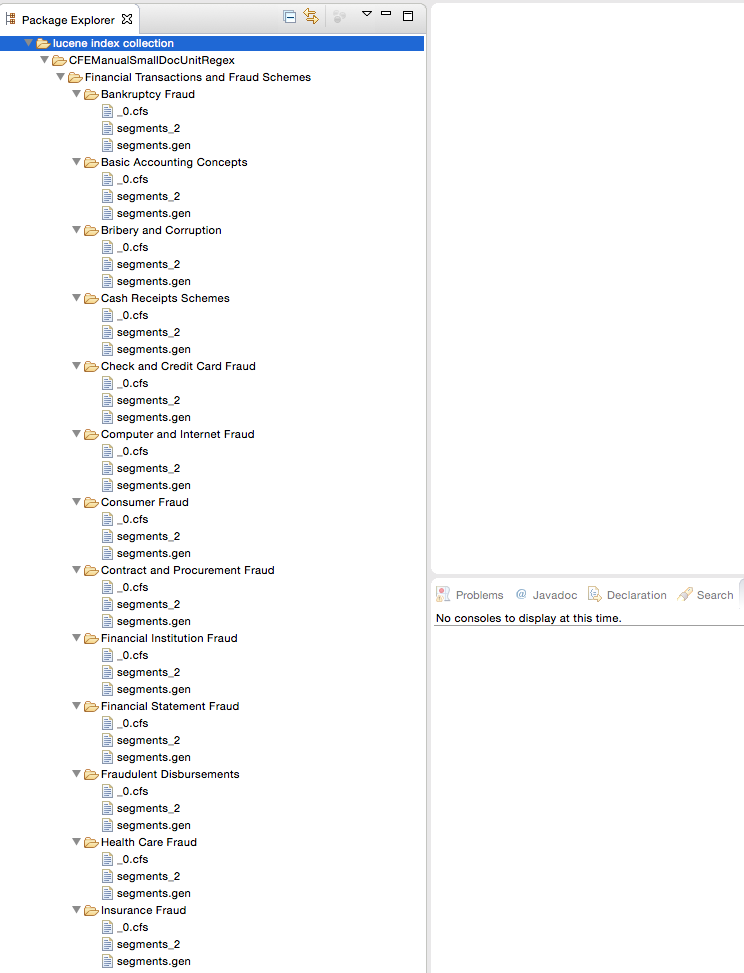
\includegraphics[width=125mm, height=200mm]{lucene_indexes.png}
\caption{Lucene Indexes for a Portion of the Question Sections}
\label{fig:lucene_indexes}
\end{figure}



\section{Analysis Tools for Algorithm Development}

As outlined in prior chapters, the goal of the CFE agent is to answer questions correctly while providing justification for those answers.  As algorithms were developed toward this end, and in particular, as we attempted to refine the accuracy of the agent by making its search functionality more fine-grained, it was determined early in the process that one of the most critical pieces of information was to understand how to target each type of question - What features for a given type of question could be exploited when searching for an answer?  Specifically, how does the answer present itself in the manual to a question of a given type?  Is it contained in a single document, or multiple documents?  Are terms found in the options commonly found in the contents of the document, or are they found in the title?  Depending on the answer, how often is that the case?  Is it always true, or only sometimes?  Tools that aided in this investigation were critical to the development of ``smarter'' algorithms.  

At a macro level, the profiler component, developed for Version 1 of the agent provided an initial analysis tool.  As discussed, it supplied a breakdown of question by macro-features, as well as the success rate of the initial algorithms created for that version.  And here in Version 2, the profiler would be used again.  However, analysis at a greater level of detail was needed.

One component, called the Question Server, was created to at least partially meet this need.  Simple in concept, it would select/pose to the agent only the questions of a particular profile, whether the desired profile be a definition question, a long answer question, and so on.  This provided a means for zero-ing on each type of question in isolation, allowing for various theories and insights to be developed about the best approach for each question.  Fig.~\ref{fig:question_server} shows output from the Question Server for definition/NOT questions, questions whose options are a small number of words (and are thus, typically relate to a definition of a conept), and contain the term, ``not" in the stem, implying the task is to identify the ``odd man out" among the options.

A second component, called the Algorithm Tester, was created on the shoulders of the Question Server, which would demonstate the behavior of each algorithm as it was applied to each question of a given type.  This, too, was instrumental in algorithm development.

\begin{figure}
\centering
\vspace{1.0in}
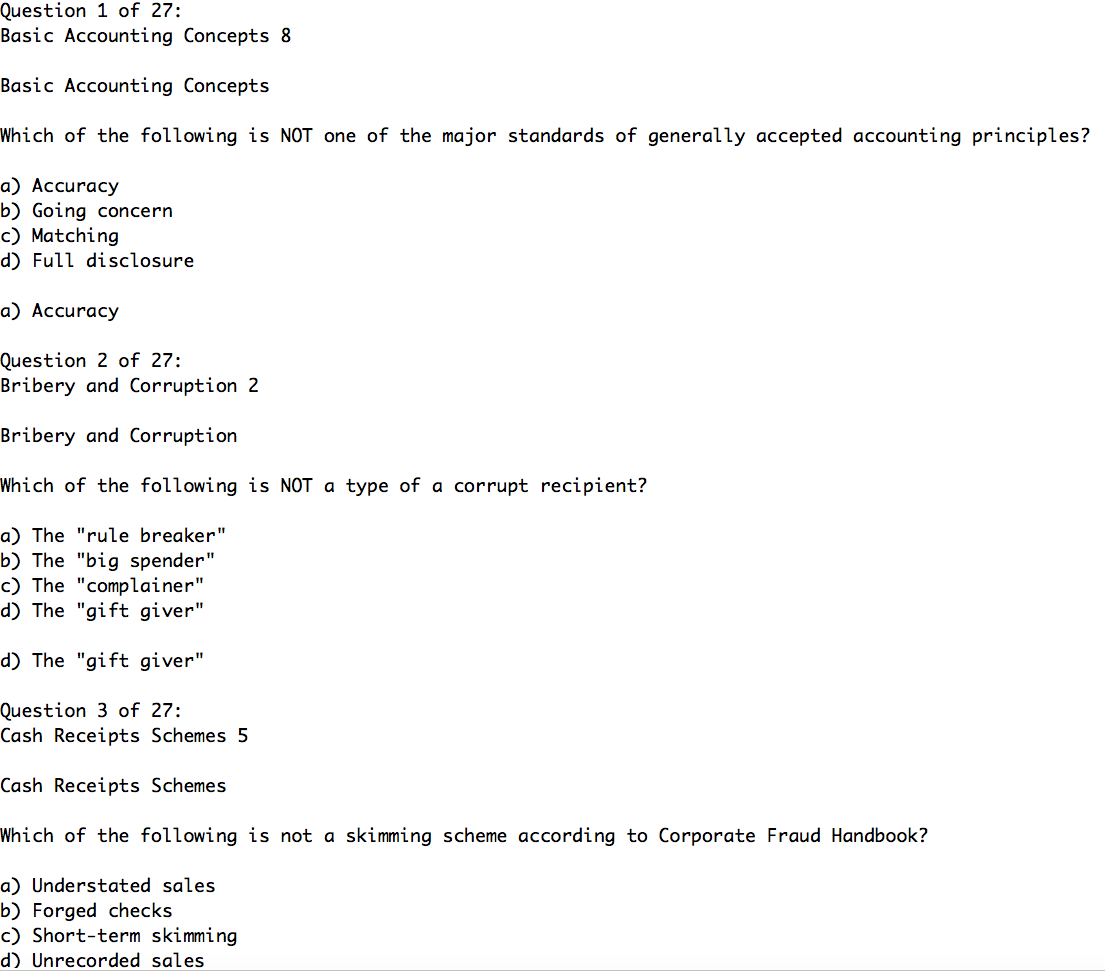
\includegraphics[width=125mm, height=125mm]{question_server.png}
\caption{Question Server Component Targeting Definition/NOT Questions}
\label{fig:question_server}
\end{figure}


\section{Algorithms for Version 2}

This section describes the algorithms implemented for Version 2 of the CFE Agent.  These algorithms rely heavily on IR, as implemented in Lucene.  They also tend to each target a particular question type, in particular, the definition questions - that is, those questions in which each of the options is only a short phrase (consisting of four words or less), and which thus are thought to be most likely the kind of question in which the stem contains a phrase that defines a given concept and the examinee must choose the correct concept from among the four options to which that phrase corresponds.  Given that a large portion of the questions in the training and test sets are some form of this type, more refined algorithms that target this type of question appeared to be a wise choice for where to focus our development efforts.

\subsection{Concept Match Version 1}

Concept Match Version 1 leverages IR on both the question stem and on each of the options in order to determine the one that fits best with the stem.  The essence of the algorithm is to first, conduct an IR query against the document collection based on the terms of the question stem, then, conduct a query based on the terms of each of the question options, and finally, select the option whose return set has the ``best overlap" with the return set for the question stem.  How do we define ``best overlap"?  For the purpose of this algorithm, a return set with ``best overlap" is the return set that includes the document that occurs in the return set of question stem query and posseses a score higher in that return set that is greater than any other document in the return sets of the other option queries.

Consider an example.  Fig.~\ref{fig:concept_match_v1_example} shows a Bankruptcy Fraud definition question.  (Although the criterion for being a definition question has only the naive requirement that all options be no more than 4 words, this example demonstrates how this criterion is often sufficient for properly categorizing this type of question, since this question really \emph{is} a definition-type question.)  The justification by the agent shows its reasoning - First, it shows the return set for each option of the four options in the question, including for each document its title, id (automatically assigned by the Lucene indexing component), and score.  (This example is particularly convenient as each option has the simplifying characteristic of at most one return document in its return set.  This is not always the case.)  Next, the agent shows return set for the query based on its stem, ``a person who holds a perfected security interest against a person filing bankruptcy".  The return set is sorted by decreasing score.  Now, the option Secured creditor option has a result set that includes the ``SECURED CREDITOR" document (it's capitalized because that's the way it appears in the text for the manual), which possesses a higher score in the question stem return set than any of the other documents in the return sets for the other options.  (In this particular case, it's also \emph{the} high scoring document in the question stem return set, although this fact is not a requirement of the algorithm.)  This means that the ``best overlap" is the ``SECURED CREDITOR" document, and as a result, the agent picks option, ``a) Secured creditor", the correct answer.

Some further details about the mechanics of this algorithm should also be mentioned here.  The algorithm conducts a query against the document collection based on the stem to return a collection of 10 documents (this number chosen arbitrarily) relating to the question.  This query is conducted against the \emph{contents} field of each document.  (Note that as alluded to previously, each document consists of four fields - a title field, a contents field, a question section field, and a path field.)  This means that when retrieving documents in response to the query, the terms in the contents field, exclusively, are used to determine the relevance of the document to that query.  The document's title and path are not considered (at least not in this algorithm).  It should also be noted that before conducting the query, functional phrases including ``is referred to as", ``are referred to as", ``which of the following", and so on, were removed from the stem as they do not offer semantic information about the nature of the question.  Also, the words of the question stem were stemmed just as the terms in the contents field of each document were during the indexing process.  This is necessary in order for the scoring to work properly.  

As for the queries based on each of the question options, they are executed against the \emph{title} field of each of the documents.  So, in order for a document to be found to match well to an option, it must have one or more terms in its \emph{title} in common with those of the option.  This greatly narrows the range of documents that produce high ranked hits, and this was by design.  It was noticed that on more than a few questions, the options map nicely to subsections whose titles align closely with the options.  Unfortunately, however, in the event the question options do not have sibling sections in the manual, this algorithm does not to perform well.


\begin{figure}
\centering
\vspace{1.0in}
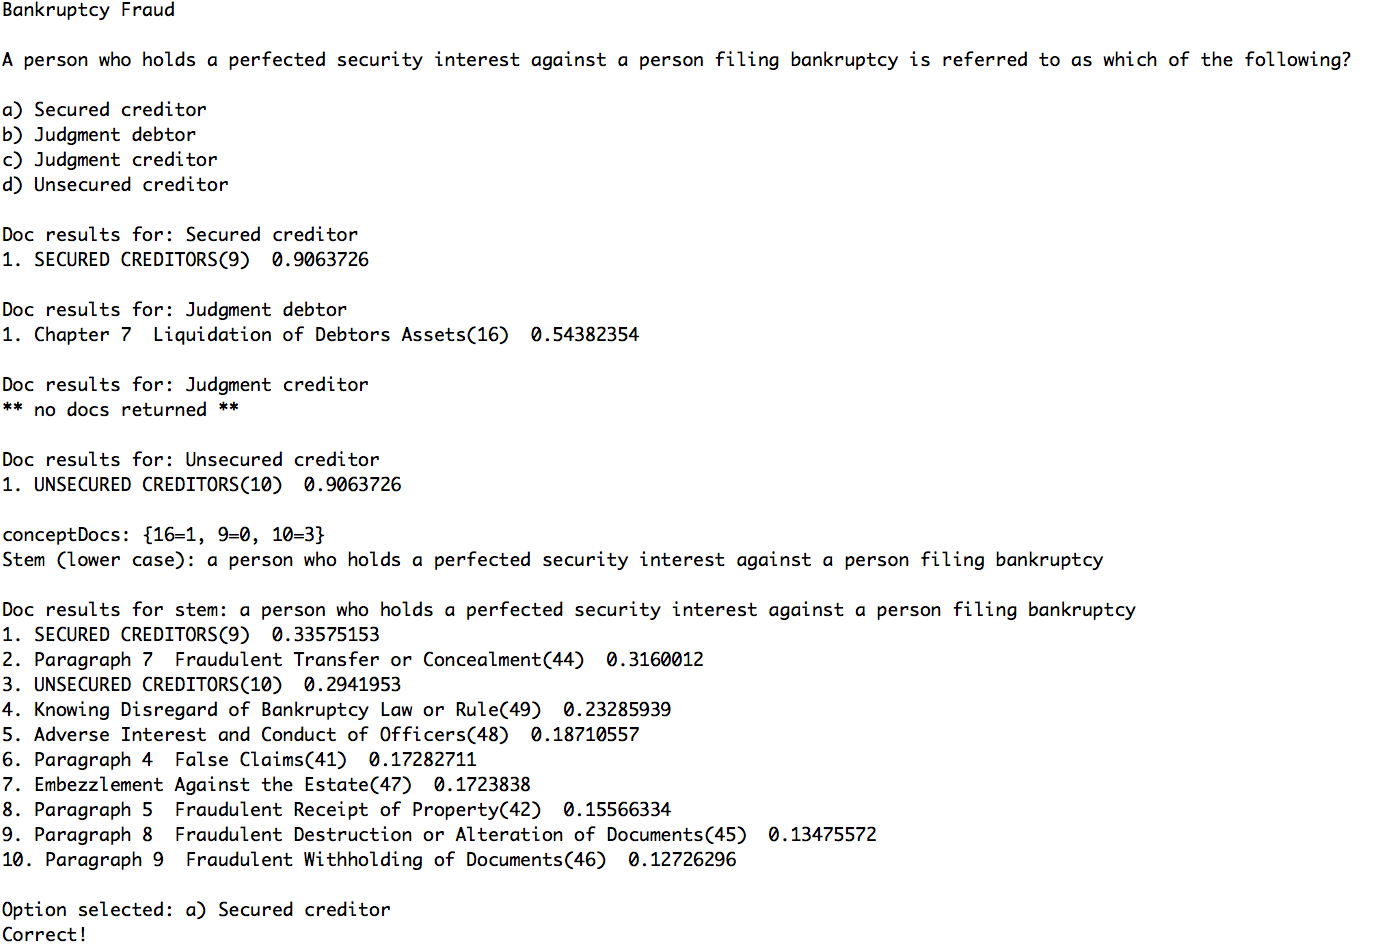
\includegraphics[width=125mm, height=125mm]{concept_match_v1_example.png}
\caption{Concept Match V1 Example}
\label{fig:concept_match_v1_example}
\end{figure}


\subsubsection{Agent Justification for Selected Answer}

Notice, in the above example, that the agent shows its reasoning for its argument.  By giving the scored return set for the question stem, and for each option, the agent provides the detail for its argument for the option it selects.  It is clear from the detailed output that among the documents in the returns set for the question stem query and among the set of documents in the return sets for the question options queries, there are two documents that appear in both - SECURED CREDITORS, (id = 9) and UNSECURED CREDITORS (id = 10).  Since the SECURED CREDITORS document earns a higher vectorization match score of 0.3375, the reasoning for selecting the Secured creditors, option a, is clear.

\subsubsection{Concept Match V1 Performance}

Finally, we look at the performance of the Concept Match Version 1 algorithm.  Fig.~\ref{fig:concept_match_v1_training_set_results_def} shows output from the algorithm tester tool described above, showing that among the 150 questions in the training set that were classified as strictly definition questions, (there were others that met the criterion for a definition question, but were classified in different but related categories, such as in the definition/not category, or definition/except category), this algorithm correctly answered 56 questions, or 37.3\% -- not an outstanding rate.  In fact it is lower than the rate of the Version 1 agent on these questions (41.3\%) using the maximum frequency algorithm based on the much shallower breakdown of the CFE manual into question sections.  However, these results also show that for 46 questions this algorithm produced no answer at all.  This was because the laser-focused question option queries against the title field of the documents in some cases returned 0 documents for \emph{all} options, thereby causing the algorithm to fail.  Fig.~\ref{fig:concept_match_v1_financial_statement_fraud_9} shows an example of this scenario.  With no documents in the set of return sets for the option queries, the algorithm has no other choice than to return -1, (for no option selected).  In the next algorithm, Concept Match V2, however, this issue is addressed.


\begin{figure}
\centering
\vspace{1.0in}
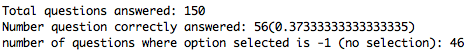
\includegraphics[width=75mm, height=15mm]{concept_match_v1_training_set_results_def.png}
\caption{Performance of Concept Match V1 on Definition Questions}
\label{fig:concept_match_v1_training_set_results_def}
\end{figure}

\begin{figure}
\centering
\vspace{1.0in}
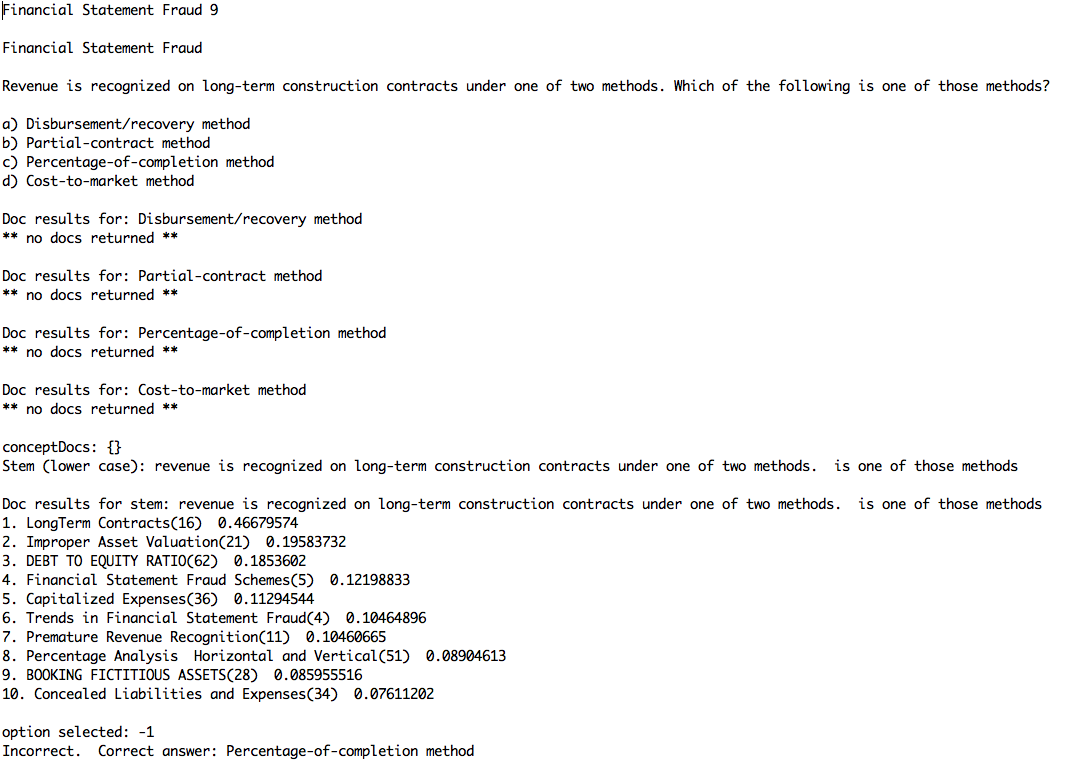
\includegraphics[width=125mm, height=125mm]{concept_match_v1_financial_statement_fraud_9.png}
\caption{Concept Match V1: An Example Where No Docs Are Returned for Options}
\label{fig:concept_match_v1_financial_statement_fraud_9}
\end{figure}


\subsection{Concept Match Version 2}

Concept Match Version 2 extends Concept Match V1 by addressing two major concerns.  The first is the situation outlined above in which for the query options no documents are returned because of the tight focus of the queries on the title field.  In Concept Match V2, if this scenario occurs, the options docs set is rebuilt, but instead of searching on the title field, the the search is performed on the contents field, thus, loosening the focus of the query resulting in a greater likelihood of documents in the return set that also occur in the question stem return set.  

The two figures, Fig.~\ref{fig:concept_match_v2_financial_statement_fraud_9_1} and Fig.~\ref{fig:concept_match_v2_financial_statement_fraud_9_2}  show the output for Concept Match V2 for the same example as  Fig.~\ref{fig:concept_match_v1_financial_statement_fraud_9} shows for Concept Match V1.  Again, this output shows the failure to return any documents or the option queries against the title field.  But whereas the V1 algorithm gives up and returns -1, V2 redoubles its efforts by re-issuing the same option queries against the contents field.  We see that in this example this form of recourse results in the algorithm producing the correct answer.

\begin{figure}
\centering
\vspace{1.0in}
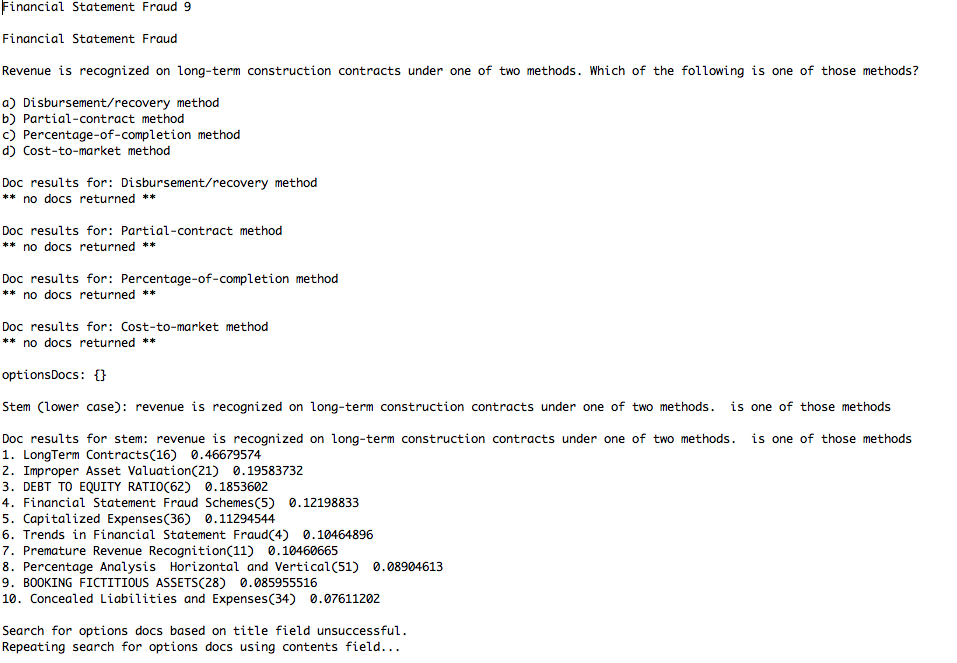
\includegraphics[width=125mm, height=125mm]{concept_match_v2_financial_statement_fraud_9_1.png}
\caption{Concept Match V2: Fixing the No Docs in Option Queries Return Sets Problem, Part 1}
\label{fig:concept_match_v2_financial_statement_fraud_9_1}
\end{figure}

\begin{figure}
\centering
\vspace{1.0in}
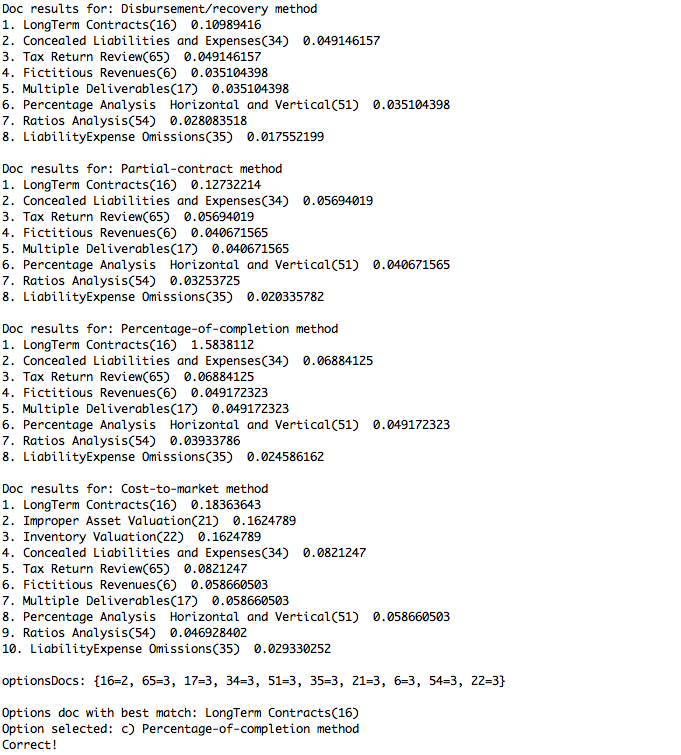
\includegraphics[width=125mm, height=125mm]{concept_match_v2_financial_statement_fraud_9_2.png}
\caption{Concept Match V2: Fixing the No Docs in Option Queries Return Sets Problem, Part 2}
\label{fig:concept_match_v2_financial_statement_fraud_9_2}
\end{figure}

The second major concern this this algorithm addresses is demonstrated by the following example shown in Fig.~\ref{fig:concept_match_v1_wrong_option_doc}.  In this case, we have a question in which the highest scoring document, (and by the way, the document which does, in fact, contain the answer to this question), ``The Business Profile Analysis", (id = 38), in the question stem return set is returned for \emph{two} options - option b, Preparing the business profile, and option c,  Preparing the vertical analysis.  Because Concept Match V1 simply loads these documents into the concept documents hash map in order by option, document 38 is \emph{initially} mapped to option b (the correct answer).  But then, this mapping is overwritten with a mapping to option c.  We can see this association in the display of the contents of the concept docs hash map, (the line in the output that starts with ``conceptDocs:"), in which we see the key/value association, 38=2, signifying that document 38 is associated with option 2 (i.e., option c; note that the option ids are 0-based, so option a is 0, option b is 1, option c is 2, and option d is 3).  As a result, the agent gets this question wrong.

\begin{figure}
\centering
\vspace{1.0in}
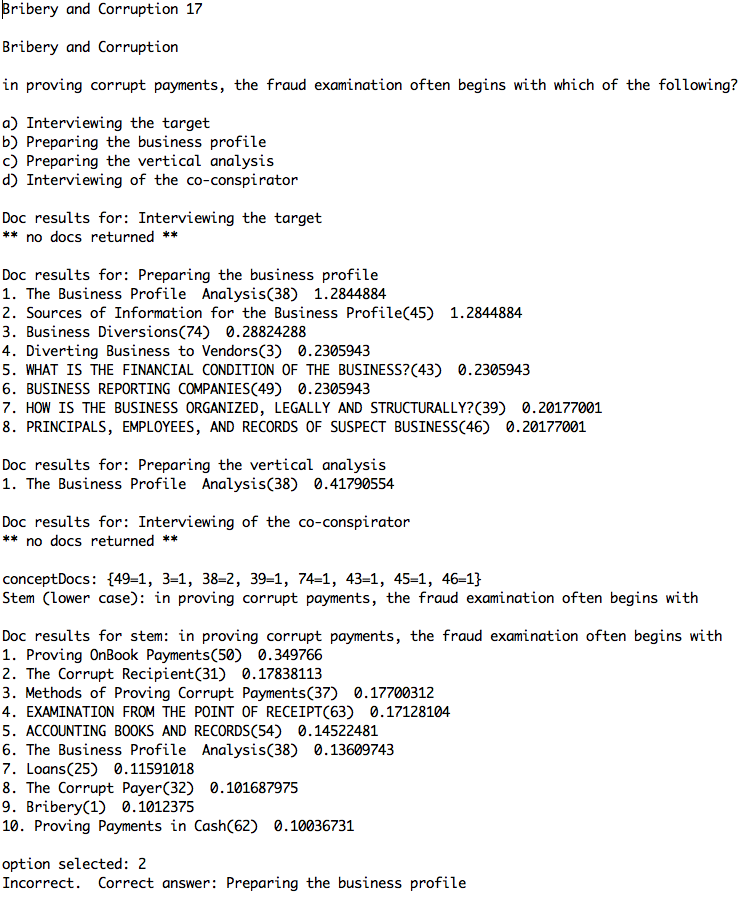
\includegraphics[width=125mm, height=125mm]{concept_match_v1_wrong_option_doc.png}
\caption{Concept Match V1: An Example Where A Document is Returned/Ranked for More than One Option}
\label{fig:concept_match_v1_wrong_option_doc}
\end{figure}

Concept Match Version 2 corrects this problem by recognizing a situation in which a document is included in multiple question-option-return-sets.  In this case, the algorithm maps the document to the option for which that document earned the highest rank score.  (Note that the lucene scoring algorithm is normalized so that scores for documents from different queries may be compared.)  Explaining this a bit more rigorously, for each concept document, $D$, with score, $S$, with respect to option $O$, if there is already an entry in the hash table for which the there is key/value pair, $D=(O',S')$, where $O'$ is a different question option and $S'$ is the score for $D$ with respect to $O'$, then scores, $S$ and $S'$ are compared, and the option whose score is maximum is chosen. If $S' > S$, then the entry with $D = (O',S')$ is left as is in the hash map. On the other hand, if $S' < S$, then the entry is overwritten with $D = (O,S)$.

For the ``Bribery and Corruption" example discussed below, we see in Fig.~\ref{fig:concept_match_v2_multiple_concept_docs} that Concept Match V2 properly associates the document, ``The Business Profile Analysis" (id = 38), with the correct option, ``b) Preparing the business profile".  The printout of the conceptDocs hash map shows the correct key/value association, 38=1, signifying that document 38 is now associated with option b, as opposed to option c.


\begin{figure}
\centering
\vspace{1.0in}
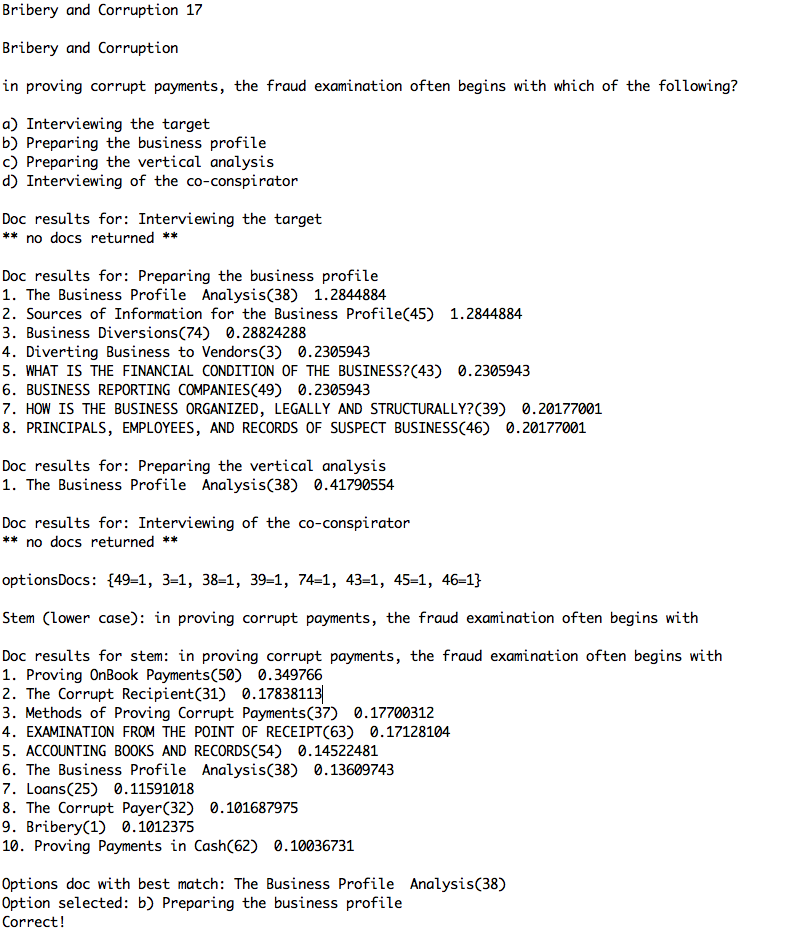
\includegraphics[width=125mm, height=125mm]{concept_match_v2_multiple_concept_docs.png}
\caption{Concept Match V2: Addressing the Problem of Multiple Options for a Document}
\label{fig:concept_match_v2_multiple_concept_docs}
\end{figure}

\subsubsection{Concept Match V2 Performance}

Next, we look at the performance of the Concept Match Version 2 algorithm on the same collection of questions which fall into the strictly defined definition-question category that were used to test Concept Match V1.  Fig.~\ref{fig:concept_match_v2_training_set_results_def} shows output from the algorithm tester shows this algorithm correctly answered 101 questions out of the collection of 150 definition questions, or 67.3\%, indicating a dramatic improvement in performance over that for Concept Match V1.  We also see that this algorithm has a much lower population of unanswered questions, (3 instead of 46), as a result of the fallback query measure incorporated into V2.



\begin{figure}
\centering
\vspace{1.0in}
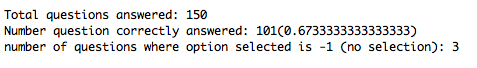
\includegraphics[width=75mm, height=15mm]{concept_match_v2_training_set_results_def.png}
\caption{Performance of Concept Match V2 on Definition Questions}
\label{fig:concept_match_v2_training_set_results_def}
\end{figure}

Fig.~\ref{fig:concept_match_v2_hypothesis_test} shows the results of a hypothesis test determining whether we can conclude a statistically significant improvement in accuracy as a result of the Concept Match V2 algorithm over that employed by Version 1 of the CFE agent, the Max Frequency algorithm, whose accuracy rate is 48.0\%.  This analysis shows that we can, in fact, draw the conclusion that Concept Match V2 offers a statistically significant improvement in performance at the 99\% confidence level.

\begin{figure}
\centering
\vspace{1.0in}
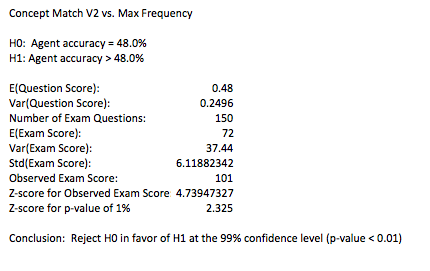
\includegraphics[width=75mm, height=60mm]{concept_match_v2_hypothesis_test.png}
\caption{Concept Match V2 vs. Max Frequency Hypothesis Test on Definition Questions}
\label{fig:concept_match_v2_hypothesis_test}
\end{figure}


\subsection{Concept Match Version 3}

Concept Match V3 attempts to build on Concept Match V2 by leveraging a behavior that was noticed in the results of the Lucene search results of the stem query.  
During development, it was noticed in a plurality of cases that  return sets for the question-stem query were headlined by a document whose score was head-and-shoulders above the rest of the docs in the return set, sometimes by a factor of three or more.  In these cases, it was commonly the case that this first-place document was, in fact, the correct document which contained the answer to the question.  So, when we have a document that hereafter will be referred to as a  ``premier document", the algorithm should focus on finding the option most closely associated with that premier document.  Concept Match V3 implements this approach by conducting queries for the options and choosing the option for which the premier document scores highest.  If no query-option queries based on the title field yield the premier document, then the algorithm repeats the query-option queries against the contents field of the document collection.  If the premier document \emph{still} does not appear in any result set, the algorithm returns -1, representing no selection.

Consider the example in Fig.~\ref{fig:concept_match_v3_example_part_1} and Fig.~\ref{fig:concept_match_v3_example_part_2}.  The question stem query for this ``Criminal Prosecutions for Fraud" question returns a result set in which the ``Arraignment" document, (id=12), with a score of 0.4654 outscores the next place document, ``Sentencing" (id=45) by a facor of more then 2.5x.  The algorithm, therefore,  categorizes this document as a premier document, and thus approaches the option selection process by attempting to find the option whose query result ranks this document higher than that for any other option.  In this example, we see that for the option queries based on the title field, the result sets are thin and there's no match to the premier document.  In this case, the algorithm re-issues the option queries, but this time casts a wider net by going aginst the contents field of each document in the collection.  In Fig.~\ref{fig:concept_match_v3_example_part_2}, we see that this approach prevails -- the result set for the correct answer, option b, the Alford plea, includes the Arraignment document.  Further, we see that although this document appears in the result sets for other options' queries, it scores highest for the Alford plea option.

\begin{figure}
\centering
\vspace{0.75in}
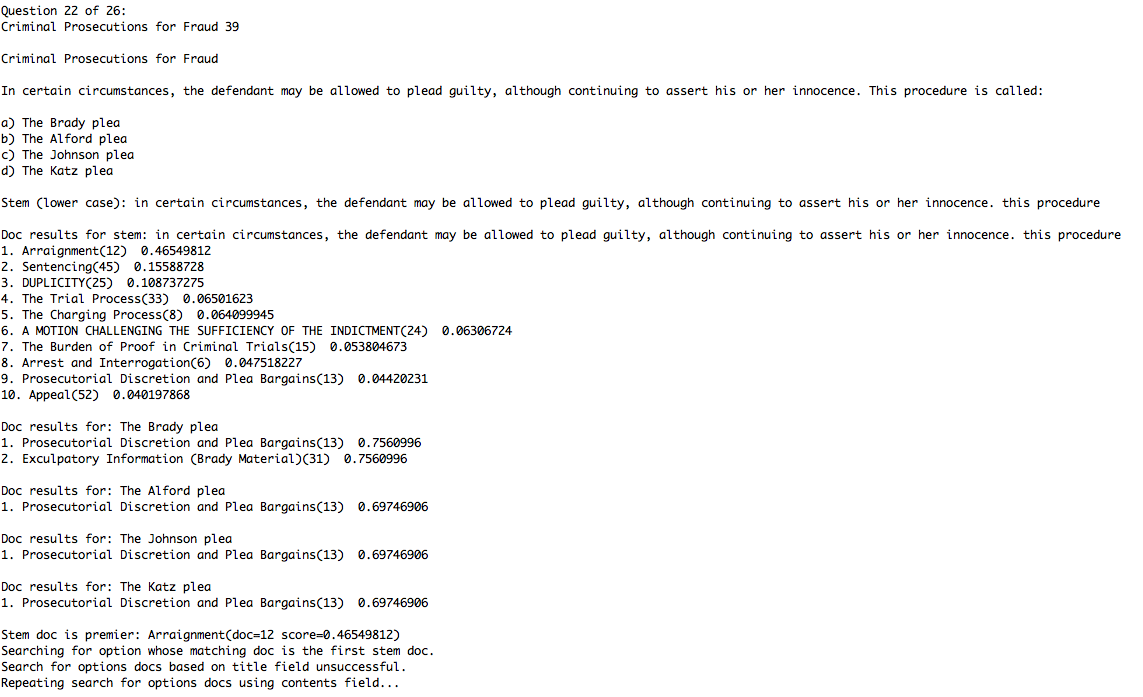
\includegraphics[width=125mm, height=125mm]{concept_match_v3_example_part_1.png}
\caption{Concept Match V3 Example - Part 1}
\label{fig:concept_match_v3_example_part_1}
\end{figure}

\begin{figure}
\centering
\vspace{0.75in}
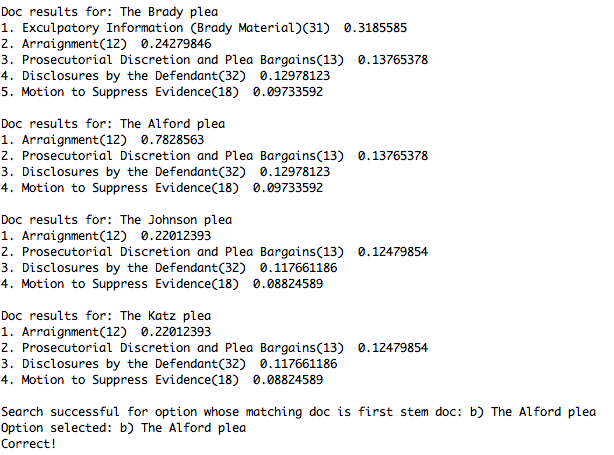
\includegraphics[width=125mm, height=125mm]{concept_match_v3_example_part_2.png}
\caption{Concept Match V3 Example - Part 2}
\label{fig:concept_match_v3_example_part_2}
\end{figure}

Fig.~\ref{fig:concept_match_v3_example_document} shows the ``Arraignment" document.  It provides a couple of key insights as to the behavior of the algorithm on this particular question.  First, we notice that the answer to the question is provided on lines 39 through 42.  The brief segment shown here concerning a description of the Alford plea suggests (and, in fact, it turns out to be the case upon further checking) that there is no document in the collection specifically dedicated to (and whose title field would be) the Alford plea.  Second, a cursory examination of this document reveals that there are number of occurrences of the term, ``plea" throughout the document which would explain why this document appears in the result set for not only the Alford plea option, but also for the Brady plea, Johnson plea, and Katz plea options.  However, the name, ``Alford" is the only one of these names mentioned in this document, and this explains why for the Alford plea option, this document scores significantly higher than for any other option.

\begin{figure}
\centering
\vspace{0.75in}
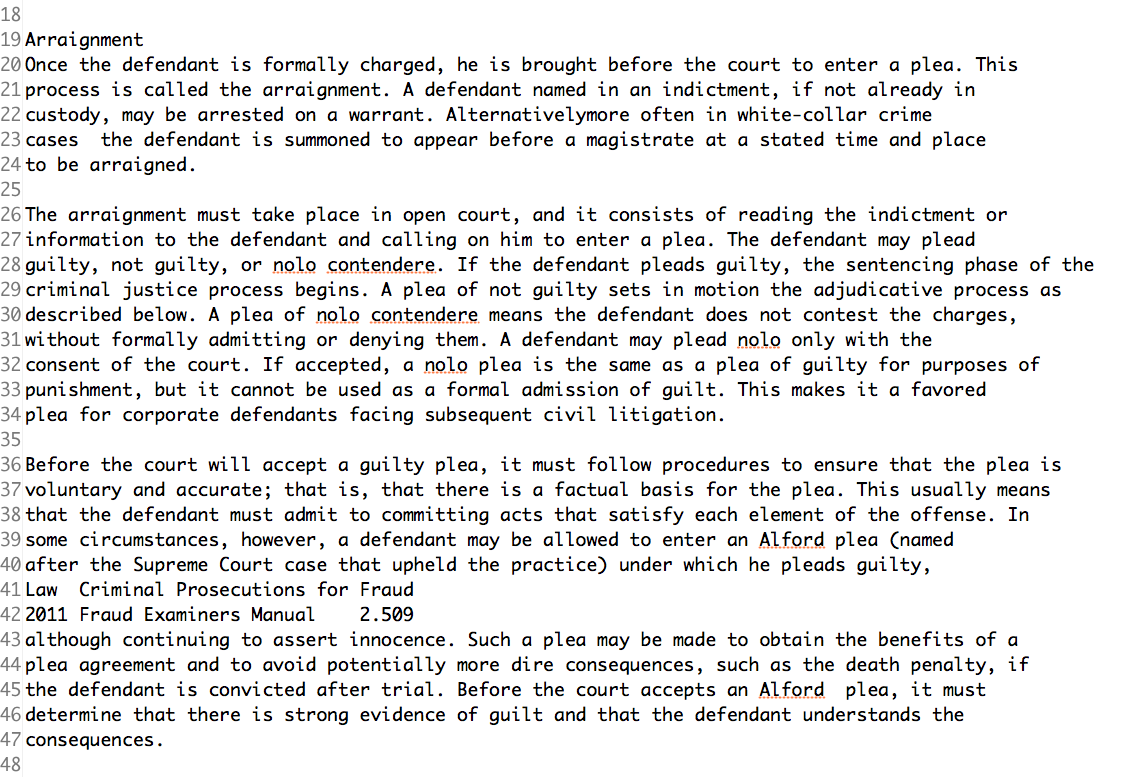
\includegraphics[width=125mm, height=125mm]{concept_match_v3_example_document.png}
\caption{The Arraignment Document}
\label{fig:concept_match_v3_example_document}
\end{figure}


\subsection{Concept Match V3 Performance}

Fig.~\ref{fig:concept_match_v3_training_set_performance} shows the performance of the Concept Match V3 algorithm on the 150 definition-type questions of the training set.  It shows that V3 improves on V2 slightly, getting 105 question correct compared with V2's 101.  However, this improvement is not significant enough to be statistically significant at the 99\% level, as the figure~\ref{fig:concept_match_v3_hypothesis_test} shows.  Nonetheless, the fact that V3 outpaces V2 means that the CFE agent will use V3 over V2 when confronted with a definition-type question, (and, as we'll see later, the agent will use this algorithm on other types of questions as well).  And finally, lest we forget, compared with Version 1 of the agent, this algorithm extends the gains we achieved with Concept Match V2 that were, themselves, found to be statistically significant relative to Version 1 of the CFE agent.

\begin{figure}
\centering
\vspace{0.75in}
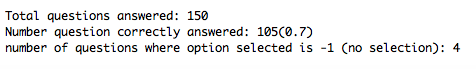
\includegraphics[width=75mm, height=15mm]{concept_match_v3_training_set_performance.png}
\caption{Performance of Concept Match V3 on Training Set}
\label{fig:concept_match_v3_training_set_performance}
\end{figure}



\begin{figure}
\centering
\vspace{0.75in}
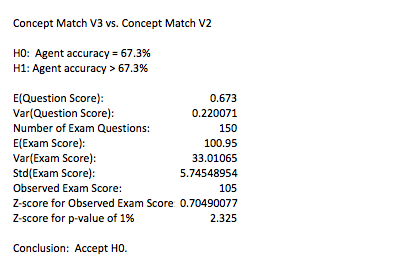
\includegraphics[width=75mm, height=60mm]{concept_match_v3_hypothesis_test.png}
\caption{Concept Match V3 vs. V2 Hypothesis Test on Definition Questions}
\label{fig:concept_match_v3_hypothesis_test}
\end{figure}



\subsection{Concept Match NOT}

Concept Match NOT extends the logic of Concept Match V3, but turns it on its head to handle questions of the type, ``Which of the following is NOT ...'', where for the phrase that follows, all options are true except for one, and of course, the agent must choose that option to correctly respond to the question.  An example of a question of this type is ``Which of the following is NOT a plea a defendant may enter at an arraignment?"
Concept Match NOT takes an approach that inverts the over-arching approach of the algorithms we've discussed above.  Instead of looking for the option for which there's the greatest affinity between option query result sets and the question stem result set, Concept Match NOT find the option whose result set has the least affinity.  

Fig.~\ref{fig:concept_match_not_example_part_1} and Fig.~\ref{fig:concept_match_not_example_part_2} show an example of this algorithm at work.  First, as we saw in the agent's justification in earlier algorithms, we see the result set for the question stem query, and then those for the option queries.  The agent then sets about attempting to map the overlap between the question stem result set and the option result sets by building two hash maps.  The first one, the ``docOptionScores" map, associates each document among the option query result sets with the the option for which that document earned the highest score.  The algorithm then utilizes this data to construct the second hash map, ``optionScoreDocs", which consists of option/document key/value pairs for which the documents are present in both the ``docOptionScores" map and in the question stem result set.  Using this data structure, the agent makes a selection; specifically, it selects the option whose document has the weakest affinity with the question stem result set.  In this case, that's option d, skimming, since this option has no representation in the optionScoreDocs data structure, implying it has no documents that overlap with the result set of the question stem.  (Looking closely, we see that whereas all of the other option queries have result sets that are non-empty, the the result set for the skimming option has no documents, and so, it's reasonable that it has the weakest affinity with the question stem.) 



\begin{figure}
\centering
\vspace{0.75in}
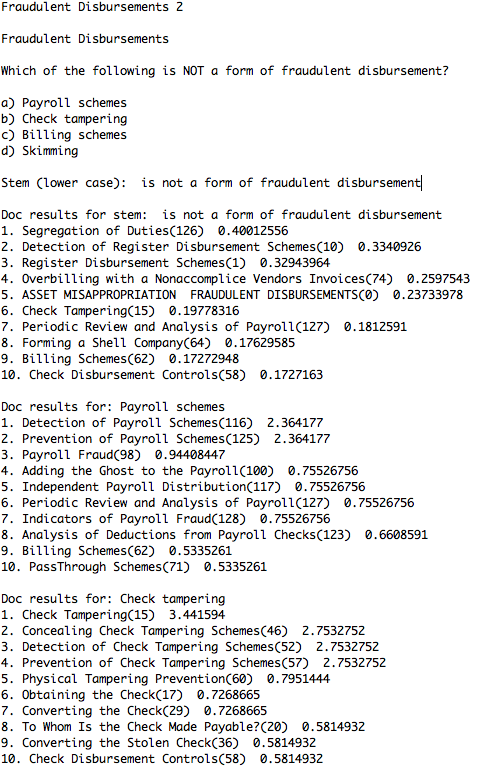
\includegraphics[width=125mm, height=125mm]{concept_match_not_example_part_1.png}
\caption{Concept Match Not Example - Part 1}
\label{fig:concept_match_not_example_part_1}
\end{figure}

\begin{figure}
\centering
\vspace{0.75in}
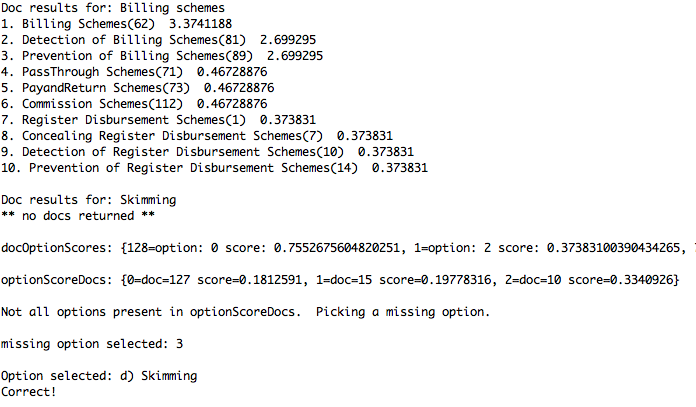
\includegraphics[width=125mm, height=90mm]{concept_match_not_example_part_2.png}
\caption{Concept Match Not Example - Part 2}
\label{fig:concept_match_not_example_part_2}
\end{figure}

\subsection{Performance of the Concept Match NOT on the Training Set - Definition/NOT Questions}

Fig.~\ref{fig:concept_match_not_training_set_performance} shows the performance of the Concept Match NOT algorithm on Definition/NOT questions in the training set - 8 out of 27 correct, or 29.6\%.  It is not unreasonable to expect that this algorithm would show weaker performance than its inverted cousin, Concept Match V3, as discovering the negative, as we are attempting to do in the case for this question type, is difficult to do.  In fact, we cannot reject the null hypothesis that this algorithm performs any better on Definition/NOT questions than random guessing, as shown in Fig.~\ref{fig:concept_match_not_hypothesis_test}.  Further investigation is required to refine this algorithm or to take a different approach with these types of questions altogether.


%However, even with that disadvantage, the Concept Match Not algorithm shows statistically significant improvement over random approach at the 99\% confidence level.  Note, we compare this algorithm to random selection because in Version 1 of the CFE Agent we observe that no algorithm actually did any better than random selection for this type of question, refer to Fig.~\ref{fig:version_1_training_set_results_not}.

\begin{figure}
\centering
\vspace{0.75in}
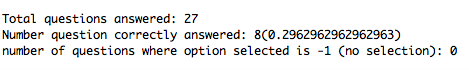
\includegraphics[width=75mm, height=13mm]{concept_match_not_training_set_performance.png}
\caption{Performance of Concept Match Not on Training Set - Definition/NOT Questions}
\label{fig:concept_match_not_training_set_performance}
\end{figure}

\begin{figure}
\centering
\vspace{0.75in}
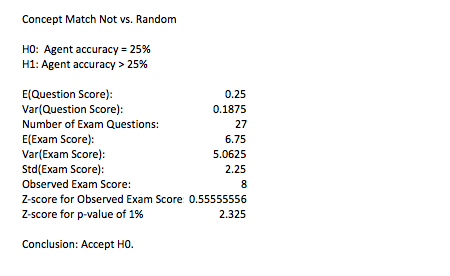
\includegraphics[width=75mm, height=60mm]{concept_match_not_hypothesis_test.png}
\caption{Concept Match Not vs. Random Hypothesis Test on Definition/Not Questions}
\label{fig:concept_match_not_hypothesis_test}
\end{figure}




\subsection{Concept Match NOTA}

Concept Match NOTA leverages the logic in Concept Match V3 for concept matching, and extends it for addressing definition questions in which the last option is ``none of the above''.  Hereafter, we'll refer to such questions as NOTA questions.

The first concern to investigate in developing this algorithm was the frequency with which the ``none of the above" option was actually the correct response in NOTA questions.  In order to determine this, we developed a trivial algorithm, called the None Of the Above Algorithm, which simply selects the last option, that is, the ``none of the above" option, always.  Then, we ran this algorithm on all 162 NOTA questions in the training set.  The ratio of the correctly answered questions for this algorithm gave us our answer.  Fig.~\ref{fig:nota_training_set_performance} shows the performance results.  We see that the ``none of the above" option is under-represented as a correct answer, serving as the correct answer only 7.4\% of the time.  Whereas we'd expect that it should be the correct answer 25\% of the time, it is, in fact, drastically under-represented as the correct answer.  This served as the inspiration for the simplistic but strategic approach of this algorithm - simply remove the ``none of the above option" as one of the possible options and select from the remaining three options (using the logic of Concept Match V3).

\begin{figure}
\centering
\vspace{0.75in}
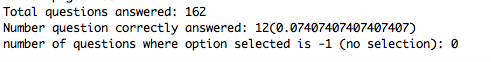
\includegraphics[width=75mm, height=13mm]{nota_training_set_performance.png}
\caption{Performance of NOTA Algorithm on NOTA Questions}
\label{fig:nota_training_set_performance}
\end{figure}


Fig.~\ref{fig:concept_match_nota_example} shows an example of the execution of this algorithm.  The agent collects the result set for the question stem query, notices that this question is a NOTA question and thus, removes the ``none of the above" option from its set of options, infers from the score of the ``Quiet Rooms" document (id=171) relative to that of the second place document that its a premier document, and picks the option for whose query scores the ``Quiet Rooms" document higher than any other option.  This leads to the correct selection of a) Quiet Rooms.


\begin{figure}
\centering
\vspace{0.75in}
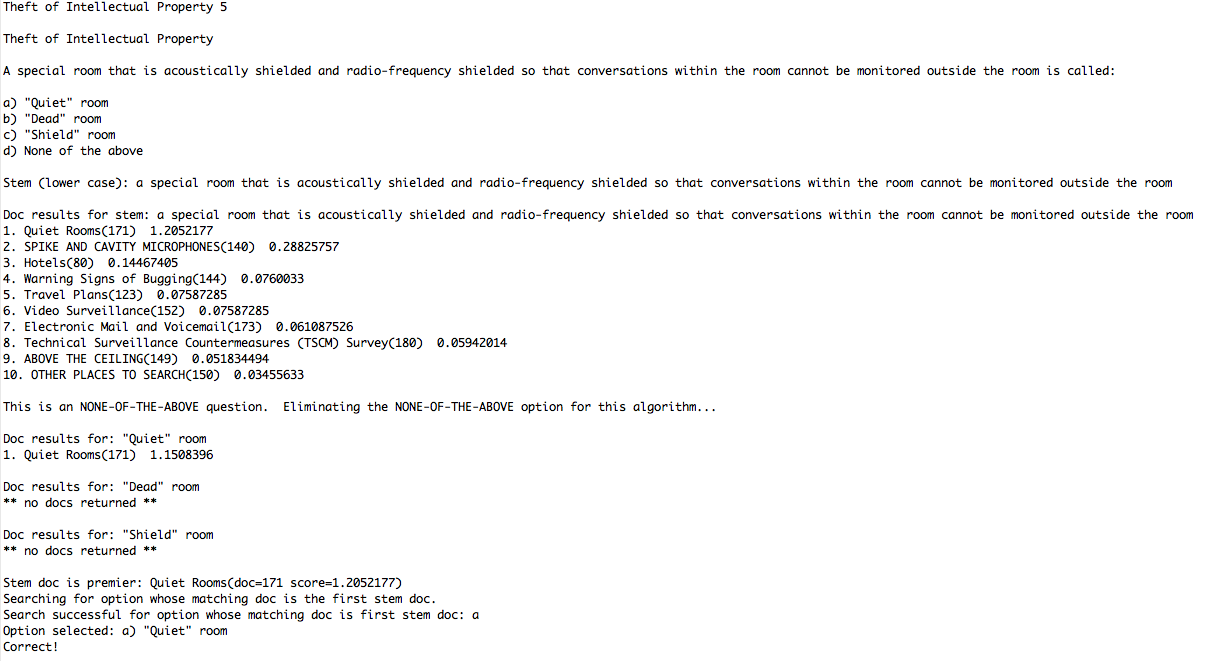
\includegraphics[width=125mm, height=100mm]{concept_match_nota_example.png}
\caption{Concept Match NOTA Example}
\label{fig:concept_match_nota_example}
\end{figure}

\subsection{Performance of Concept Match NOTA}

Fig.~\ref{fig:concept_match_nota_training_set_performance} shows the performance of this algorithm on the Definition/NOTA questions at 65.4\% accuracy.  Fig.~\ref{fig:concept_match_nota_hypothesis_test} shows a hypothesis test of this algorithm against the Max Frequency algorithm which had the best results in the CFE Agent Version 1.  Since Max Frequency showed results of 56.5\% on 162 questions, the results of Concept Match NOTA were \emph{just short} of showing statistically significant improvement at the 99\% confidence level.  However, notice that the improvement posted by this algorithm \emph{is} significant at the 98\% confidence level.  Given this, we incorporate this algorithm into the agent as part of its enhanced suite of tools of Version 2.

\begin{figure}
\centering
\vspace{0.75in}
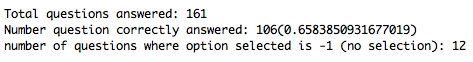
\includegraphics[width=75mm, height=13mm]{concept_match_nota_training_set_performance.png}
\caption{Performance of Concept Match NOTA on Training Set - Definition/NOTA Questions}
\label{fig:concept_match_nota_training_set_performance}
\end{figure}



\begin{figure}
\centering
\vspace{0.75in}
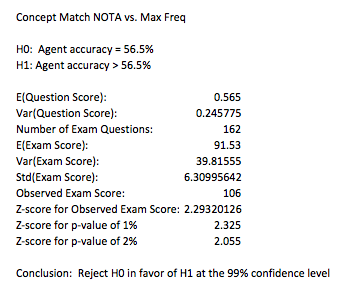
\includegraphics[width=100mm, height=75mm]{concept_match_nota_hypothesis_test.png}
\caption{Concept Match NOTA vs. Max Frequency Hypothesis Test on Definition/NOTA  Questions}
\label{fig:concept_match_nota_hypothesis_test}
\end{figure}





\section{CFE Agent Version 2 Results}

Fig.~\ref{fig:version_2_training_set_performance} summarizes the performance of the CFE Agent Version 2.  It shows that with a 70.0\% accuracy rate on definition questions, Concept Match V3 is the preferred algorithm for that question type.  And Concept Match NOT is the preferred algorithm for definition/NOT questions, even with the disappointing accuracy rate of only  29.6\%.  This algorithm also emerges as the favorite for definition/EXCEPT questions (``All of the following are .... EXCEPT ....") as well, with an accuracy rate of 46.7\%.  This is not surprising as this type of question is semantically equivalent to the Definition/NOT question, so it is reasonable for this algorithm to be the top performer for this type as well.  Finally, Concept Match NOTA is the preferred algorithm for NOTA questions, with an accuracy of 65.8\%.

%\begin{figure}
%\centering
%\vspace{0.75in}
%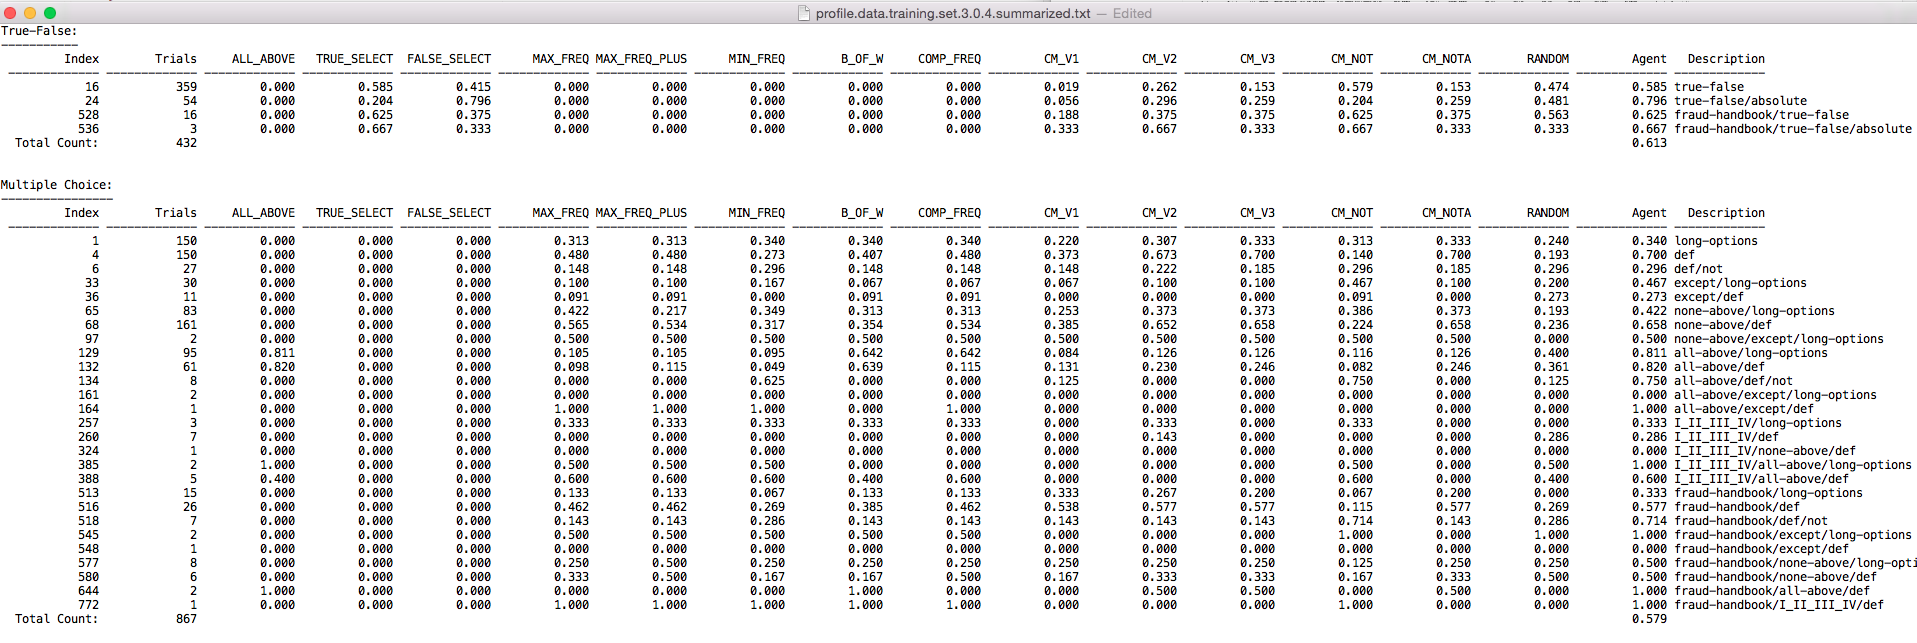
\includegraphics[width=125mm, height=100mm, angle=90]{version_2_training_set_performance.png}
%\caption{Performance of CFE Agent Version 2 on Training Set}
%\label{fig:version_2_training_set_performance}
%\end{figure}

\begin{sidewaysfigure}
\centering
\vspace{0.25in}
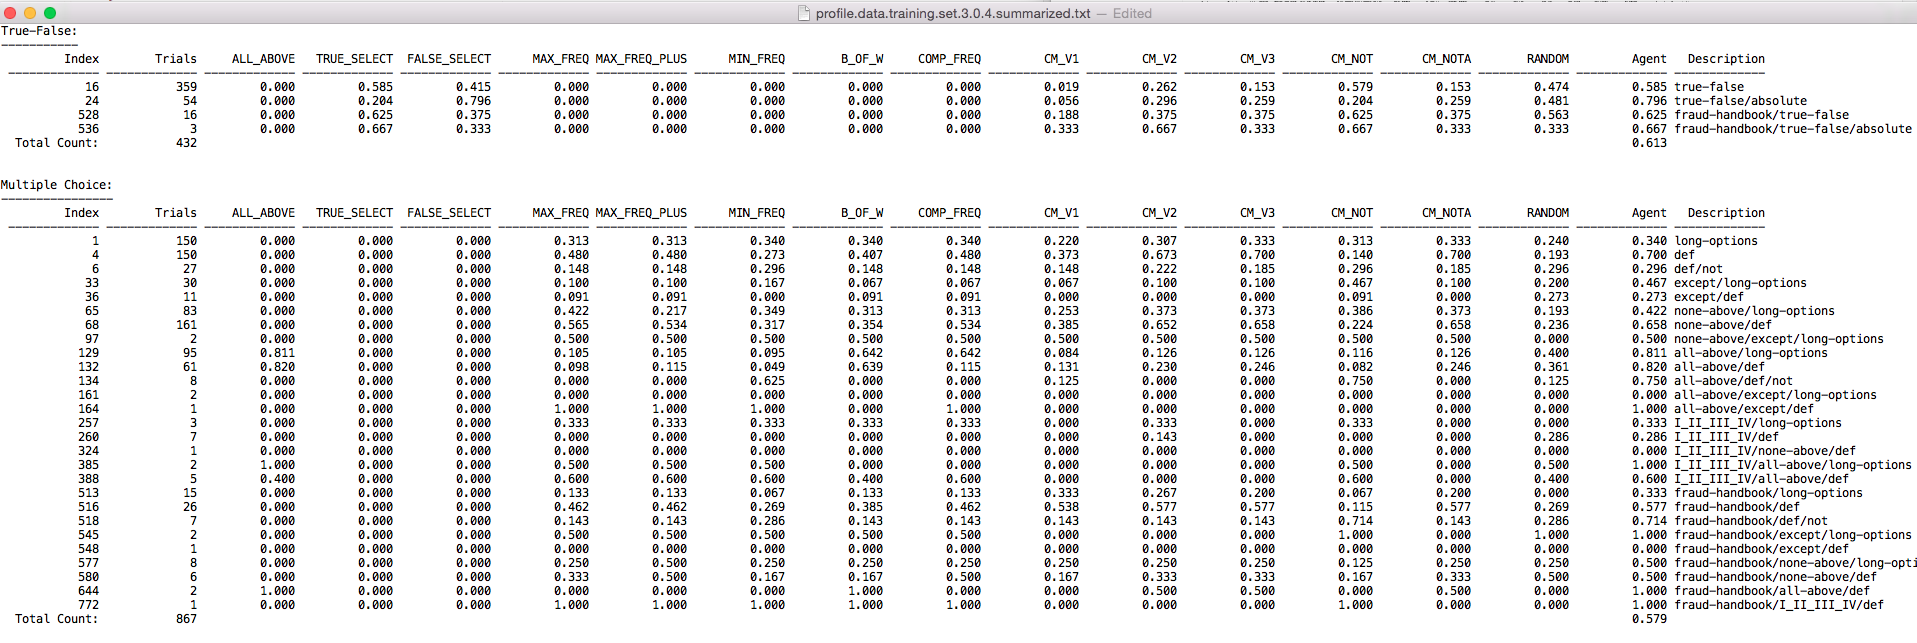
\includegraphics[width=\textwidth]{version_2_training_set_performance.png}
\caption{Performance of CFE Agent Version 2 on Training Set}
\label{fig:version_2_training_set_performance}
\end{sidewaysfigure}

Fig.~\ref{fig:version_2_multiple_choice_hypothesis_test} shows the results of a hypothesis test of the performance of the CFE Agent Version 2 on the entire battery of training set questions relative to that of Version 1.  The analysis shows the improvement for Version 2 over Version 1 to be statistically significant at the 99\% level.  This should not be surprising since the question types for which we've targeted our new algorithms, namely Definition, Definition/NOT, and Definition/NOTA , constitute a large portion of the question battery (338 of the 867 questions), as indicated by the Trials column of the table in Fig.~\ref{fig:version_2_training_set_performance}.

\begin{figure}
\centering
\vspace{0.75in}
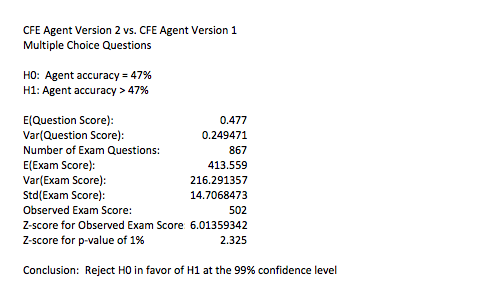
\includegraphics[width=75mm, height=60mm]{version_2_multiple_choice_hypothesis_test.png}
\caption{CFE Agent Version 2 vs. CFE Agent Version 1 Hypothesis Test on Multiple Choice Questions}
\label{fig:version_2_multiple_choice_hypothesis_test}
\end{figure}

Running the CFE Agent on the test set of 200 questions yields a score of 119 out of 200, or 59.5\%, a dramatic improvement over the 49\% of Version 1.

















